%    Copyright © 2015
%  Eduardo Candido Xavier <eduardo@ic.unicamp.br>
%
%  This work is free. You can redistribute it and/or modify it under the
%  terms of the Do What The Fuck You Want To Public License, Version 2,
%  as published by Sam Hocevar. See the COPYING file for more details.
%
%  DO WHAT THE FUCK YOU WANT TO PUBLIC LICENSE
%                   Version 2, December 2004
%
%   Copyright (C) 2004 Sam Hocevar <sam@hocevar.net>
%
%   Everyone is permitted to copy and distribute verbatim or modified
%   copies of this license document, and changing it is allowed as long
%   as the name is changed.
%
%  DO WHAT THE FUCK YOU WANT TO PUBLIC LICENSE
%   TERMS AND CONDITIONS FOR COPYING, DISTRIBUTION AND MODIFICATION
%
%      0. You just DO WHAT THE FUCK YOU WANT TO.

\documentclass[handout]{beamer}
\usetheme{metropolis}
\beamertemplatetransparentcoveredhigh

\usepackage[portuges]{babel}
\usepackage{graphicx}
\graphicspath{{./figs/}}
\usepackage{listings}
\usepackage{color}
\usepackage{hyperref}
\usepackage{xpatch}
\usepackage{moresize}
\usepackage[outputdir=build]{minted}

\makeatletter
\AtBeginEnvironment{minted}{\dontdofcolorbox}
\def\dontdofcolorbox{\renewcommand\fcolorbox[4][]{##4}}
\xpatchcmd{\inputminted}{\minted@fvset}{\minted@fvset\dontdofcolorbox}{}{}
\xpatchcmd{\mintinline}{\minted@fvset}{\minted@fvset\dontdofcolorbox}{}{}
\makeatother
\setminted[c]{
  linenos=true,
  breaklines=true,
  encoding=utf8,
  frame=lines,
  framerule=0.5pt,
  autogobble,
  fontsize=\small,
}
\setminted[bash]{
  linenos=true,
  encoding=utf8,
  frame=lines,
  framerule=0.5pt,
  autogobble,
  fontsize=\small
}

\newcommand{\cod}[1]{\mintinline{c}{#1}}


\definecolor{dkgreen}{rgb}{0,0.6,0}
\definecolor{gray}{rgb}{0.5,0.5,0.5}
\definecolor{mauve}{rgb}{0.58,0,0.82}


\definecolor{Purple}{HTML}{911146}
\definecolor{Orange}{HTML}{CF4A30}
\setbeamercolor{alerted text}{fg=Orange}
\setbeamercolor{frametitle}{bg=Purple}
\setbeamercolor{block body}{bg=Purple!20,fg=black}
\setbeamercolor{block title}{bg=Purple!50,fg=black}
\setbeamertemplate{blocks}[rounded][shadow=true]


\newcommand{\setcoverbg}{
  \setbeamertemplate{background}
  {
\includegraphics[width=\paperwidth,height=\paperheight]{backgrounds/coverbg}}
}
\newcommand{\setsectionbg}{
  \setbeamertemplate{background}
  {
\includegraphics[width=\paperwidth,height=\paperheight]{backgrounds/blank}}
}

\title{Programação Estruturada}
\subtitle{Estruturas condicionais}

\author{Professores Emílio Francesquini e Carla Negri Lintzmayer}
\institute{Centro de Matemática, Computação e Cognição\\ Universidade Federal do ABC}
\date{2018.Q3}

\begin{document}

\setcoverbg
\maketitle
\setsectionbg

%%%%%%%%%%%%%%%%%%%%%%%%%%%%%%%%%%%%%%%%%%%%%%%%
%%%%%%%%%%%%%%%%%%%%%%%%%%%%%%%%%%%%%%%%%%%%%%%%
%%%%%%%%%%%%%%%%%%%%%%%%%%%%%%%%%%%%%%%%%%%%%%%%
%%%%%%%%%%%%%%%%%%%%%%%%%%%%%%%%%%%%%%%%%%%%%%%%
%%%%%%%%%%%%%%%%%%%%%%%%%%%%%%%%%%%%%%%%%%%%%%%%
%%%%%%%%%%%%%%%%%%%%%%%%%%%%%%%%%%%%%%%%%%%%%%%%

\section{Comandos condicionais}

%%%%%%%%%%%%%%%%%%%%%%%%%%%%%%%%%%%%%%%%%%%%%%%%
\begin{frame}[fragile]{Comandos condicionais}

    Um comando condicional é aquele que permite decidir se um determinado bloco de comandos deve ou não ser executado, de acordo com o resultado de uma expressão relacional ou lógica.

    \begin{center}
        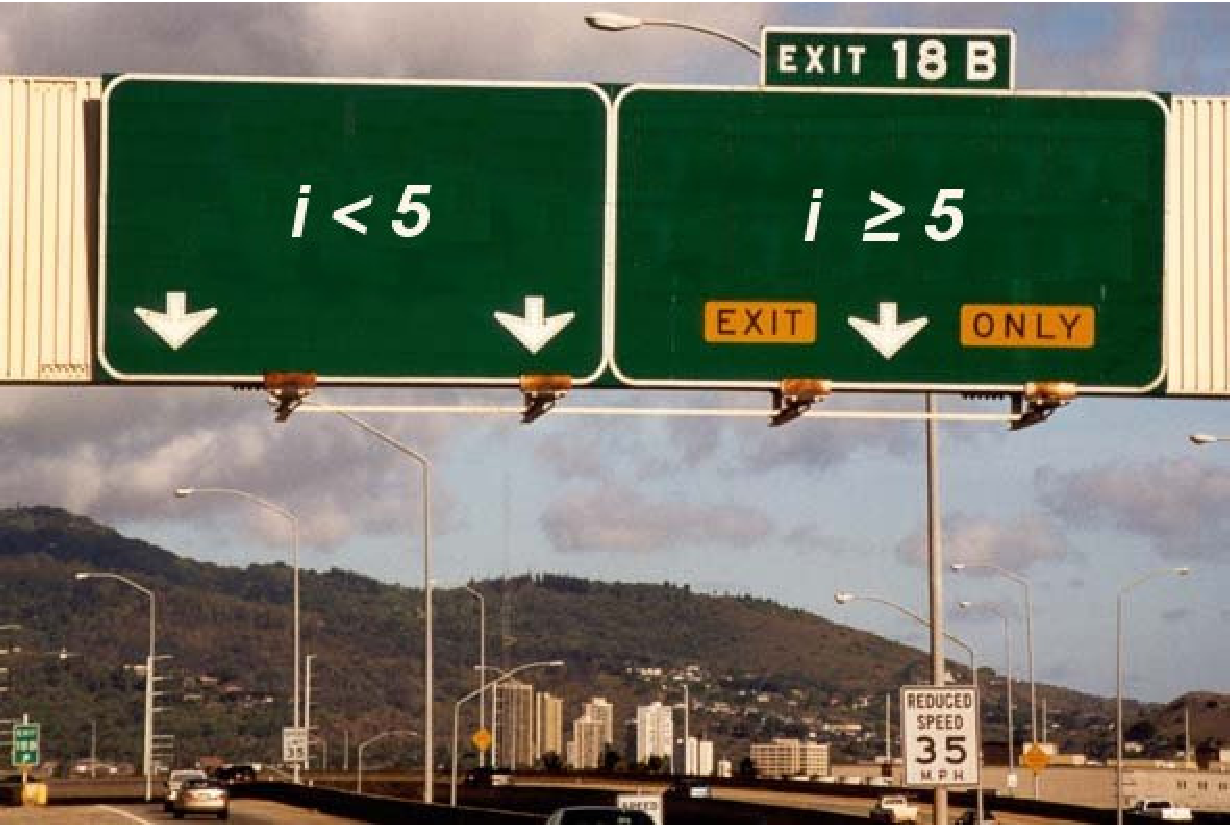
\includegraphics[width=0.7\textwidth]{figs/exit.pdf}
    \end{center}
\end{frame}

%%%%%%%%%%%%%%%%%%%%%%%%%%%%%%%%%%%%%%%%%%%%%%%%
\begin{frame}[fragile]{Bloco de comandos}

    \begin{itemize}
        \item É um conjunto de instruções agrupadas
        \item Em C, é limitado pelos caracteres {\bf \{} e {\bf \}}
    \end{itemize}

    \begin{minted}{c}
        #include <stdio.h>

        int main() { /* início do bloco de comandos */
            int a;
            a = 1;
            return 0;
        } /* fim do bloco de comandos */
    \end{minted}
\end{frame}

%%%%%%%%%%%%%%%%%%%%%%%%%%%%%%%%%%%%%%%%%%%%%%%%
\begin{frame}[fragile]{Comandos condicionais}

    O principal comando condicional da linguagem C é o {\bf if}, cuja sintaxe é

    \begin{minted}{c}
        if (expressão relacional ou lógica)
            um único comando;
    \end{minted}

    ou

    \begin{minted}{c}
        if (expressão relacional ou lógica) {
            sequência de comandos;
        }
    \end{minted}

    Os comandos são executados somente se a expressão relacional/lógica for verdadeira.
\end{frame}

%%%%%%%%%%%%%%%%%%%%%%%%%%%%%%%%%%%%%%%%%%%%%%%%
\begin{frame}[fragile]{Comandos condicionais}

    O programa abaixo determina se um valor é ímpar.
    \pause

    \begin{minted}{c}
        #include <stdio.h>

        int main() {
            int a;

            scanf("%d", &a);
            if ((a % 2) != 0) {
                printf("O valor digitado é ímpar.\n");
            }

            return 0;
        }
    \end{minted}
\end{frame}

%%%%%%%%%%%%%%%%%%%%%%%%%%%%%%%%%%%%%%%%%%%%%%%%
\begin{frame}[fragile]{Comandos condicionais}

    Lembrando como C representa os valores falso e verdadeiro, o programa anterior é equivalente ao seguinte.

    \begin{minted}{c}
        #include <stdio.h>

        int main() {
            int a;

            scanf("%d", &a);
            if (a % 2) {
                printf ("O valor digitado é ímpar.\n");
            }

            return 0;
        }
    \end{minted}
\end{frame}

%%%%%%%%%%%%%%%%%%%%%%%%%%%%%%%%%%%%%%%%%%%%%%%%
\begin{frame}[fragile]{Comandos condicionais}

    Uma variação do comando {\bf if} é o {\bf if/else}, cuja sintaxe é

    \begin{minted}{c}
        if (expressão relacional ou lógica) {
            comandos executados se a expressão é verdadeira;
        } else {
            comandos executados se a expressão é falsa;
        }
    \end{minted}
\end{frame}

%%%%%%%%%%%%%%%%%%%%%%%%%%%%%%%%%%%%%%%%%%%%%%%%
\begin{frame}[fragile]{Comandos condicionais}

    O programa a seguir determina o menor dentre dois números.

    \begin{minted}[fontsize=\footnotesize]{c}
        #include <stdio.h>
        int main() {
            int a, b;

            scanf("%d", &a);
            scanf("%d", &b);

            if (a < b) {
                printf("O menor número é: %d\n", a);
            } else {
                printf("O menor número é: %d\n", b);
            }

            return 0;
        }
    \end{minted}
\end{frame}

%%%%%%%%%%%%%%%%%%%%%%%%%%%%%%%%%%%%%%%%%%%%%%%%
\begin{frame}[fragile]{Comandos condicionais}

    Note que o {\bf if} é um comando e, como tal, pode aparecer dentro do bloco de comandos de outro {\bf if}.

    Exemplo: usando \textbf{apenas} operadores relacionais e aritméticos, vamos escrever um programa que lê um número e verifica em qual dos seguintes casos o número se enquadra:
    \begin{itemize}
        \item Par e menor que 100
        \item Par e maior ou igual a 100
        \item Ímpar e menor que 100
        \item Ímpar e maior ou igual a 100
    \end{itemize}
\end{frame}

%%%%%%%%%%%%%%%%%%%%%%%%%%%%%%%%%%%%%%%%%%%%%%%%
\begin{frame}[fragile]{Comandos condicionais}

    \begin{minted}[fontsize=\scriptsize]{c}
        #include <stdio.h>
        int main() {
            int a;

            scanf("%d", &a);

            if (a % 2 == 0) {
                if (a < 100)
                    printf("O número é par e menor que 100\n");
                else
                    printf("O número é par e maior ou igual a 100\n");
            } else {
                if (a < 100)
                    printf("O número é ímpar e menor que 100\n");
                else
                    printf("O número é ímpar e maior que 100\n");
            }

            return 0;
        }
    \end{minted}

    Se você pudesse usar operadores lógicos, como você poderia refazer este programa?
\end{frame}

%%%%%%%%%%%%%%%%%%%%%%%%%%%%%%%%%%%%%%%%%%%%%%%%
\begin{frame}[fragile]{Comandos condicionais}

    \begin{minted}[fontsize=\footnotesize]{c}
        #include <stdio.h>

        int main() {
            int a;
            scanf("%d", &a);

            if ((a % 2 == 0) && (a < 100))
                printf("O número é par e menor que 100\n");
            if ((a % 2 == 0) && (a >= 100))
                printf("O número é par e maior ou igual a 100\n");
            if ((a % 2 != 0) && (a < 100))
                printf("O número é ímpar e menor que 100\n");
            if ((a % 2 != 0) && (a >= 100))
                printf("O número é ímpar e maior que 100\n");

            return 0;
        }
    \end{minted}
\end{frame}

%%%%%%%%%%%%%%%%%%%%%%%%%%%%%%%%%%%%%%%%%%%%%%%%
\begin{frame}[fragile]{Comandos condicionais}

    \begin{minted}{c}
        if (cond1) {
            if (cond2)
                comando1;
        } else
            comando2;
    \end{minted}

    Quando o {\bf comando2} é executado?
    %\pause
    %Resposta: quando {\bf cond1} for falsa.
\end{frame}

%%%%%%%%%%%%%%%%%%%%%%%%%%%%%%%%%%%%%%%%%%%%%%%%
\begin{frame}[fragile]{Comandos condicionais}

    \begin{minted}{c}
        if (cond1) {
            if (cond2)
                comando1;
            else
                comando2;
        } else {
            if (cond3)
                comando3;
            else
                comando4;
        }
    \end{minted}

    Quando o {\bf comando4} é executado?
    %\pause
    %Resposta: quando \textbf{cond1} e \textbf{cond3} são falsas.
\end{frame}

%%%%%%%%%%%%%%%%%%%%%%%%%%%%%%%%%%%%%%%%%%%%%%%%
\begin{frame}[fragile]{Comandos condicionais}

    Use chaves e indentação para deixar claro a qual comando condicional um outro comando pertence!!

    \begin{minted}{c}
        if (cond1)
        if (cond2)
            comando1;
        else
            comando2;
    \end{minted}

    Quando o {\bf comando2} é executado?
    %\pause
    %Resposta: \textbf{if/else} é um único comando, portanto ele está dentro do primeiro \textbf{if}; logo, \textbf{comando2} é executado quando \textbf{cond1} for verdadeira e \textbf{cond2} for falsa.
\end{frame}

%%%%%%%%%%%%%%%%%%%%%%%%%%%%%%%%%%%%%%%%%%%%%%%%
\begin{frame}[fragile]{Comandos condicionais}

    Usando chaves e indentação no exemplo anterior para deixar mais claro:

    \begin{minted}{c}
        if (cond1) {
            if (cond2)
                comando1;
            else
                comando2;
        }
    \end{minted}
\end{frame}

%%%%%%%%%%%%%%%%%%%%%%%%%%%%%%%%%%%%%%%%%%%%%%%%
\begin{frame}[fragile]{Comandos condicionais}

    \begin{minipage}{0.5\textwidth}
        \begin{minted}{c}
            #include <stdio.h>
            int main() {
                int a;
                scanf("%d", &a);

                if (a > 3) {
                    if (a < 7)
                        printf("a\n");
                } else {
                    if (a > -10)
                        printf("b\n");
                    else
                        printf("c\n");
                }

                return 0;
            }
        \end{minted}
    \end{minipage}
    \begin{minipage}{0.35\textwidth}
        O que será impresso se digitarmos:
        \begin{itemize}[<+->]
            \item 5
            \item -12
            \item 9
        \end{itemize}
    \end{minipage}
\end{frame}

%%%%%%%%%%%%%%%%%%%%%%%%%%%%%%%%%%%%%%%%%%%%%%%%
\begin{frame}[fragile]{Mais sobre o comando de atribuição}

    O comando de atribuição em C é \textbf{=}.

    Em C, uma expressão de atribuição tem valor igual ao valor da variável à esquerda.

    \begin{minted}{c}
        #include <stdio.h>

        int main() {
            int a, b;
            printf("%d\n", (a = 4));
            printf("%d\n", (a = 0));
            printf("%d\n", (a = 4+5));
            printf("%d\n", (a = b = 4));
            return 0;
        }
    \end{minted}
\end{frame}

%%%%%%%%%%%%%%%%%%%%%%%%%%%%%%%%%%%%%%%%%%%%%%%%
\begin{frame}[fragile]{Comandos condicionais}

    Não confunda o comando de atribuição com o teste de igualdade (\textbf{==}), pois isto pode gerar erros!

    \begin{minted}[fontsize=\scriptsize]{c}
        #include <stdio.h>

        int main() {
            int a = 2;

            if (a = 3) {
                printf("fazer algo se a for 3\n");
            } else {
                printf("fazer algo se a não for 3\n");
            }

            return 0;
        }
    \end{minted}

    \pause
    O programa acima imprime ``fazer algo se a for 3''.
\end{frame}

%%%%%%%%%%%%%%%%%%%%%%%%%%%%%%%%%%%%%%%%%%%%%%%%
\begin{frame}{Comandos condicionais}
    \begin{center}
        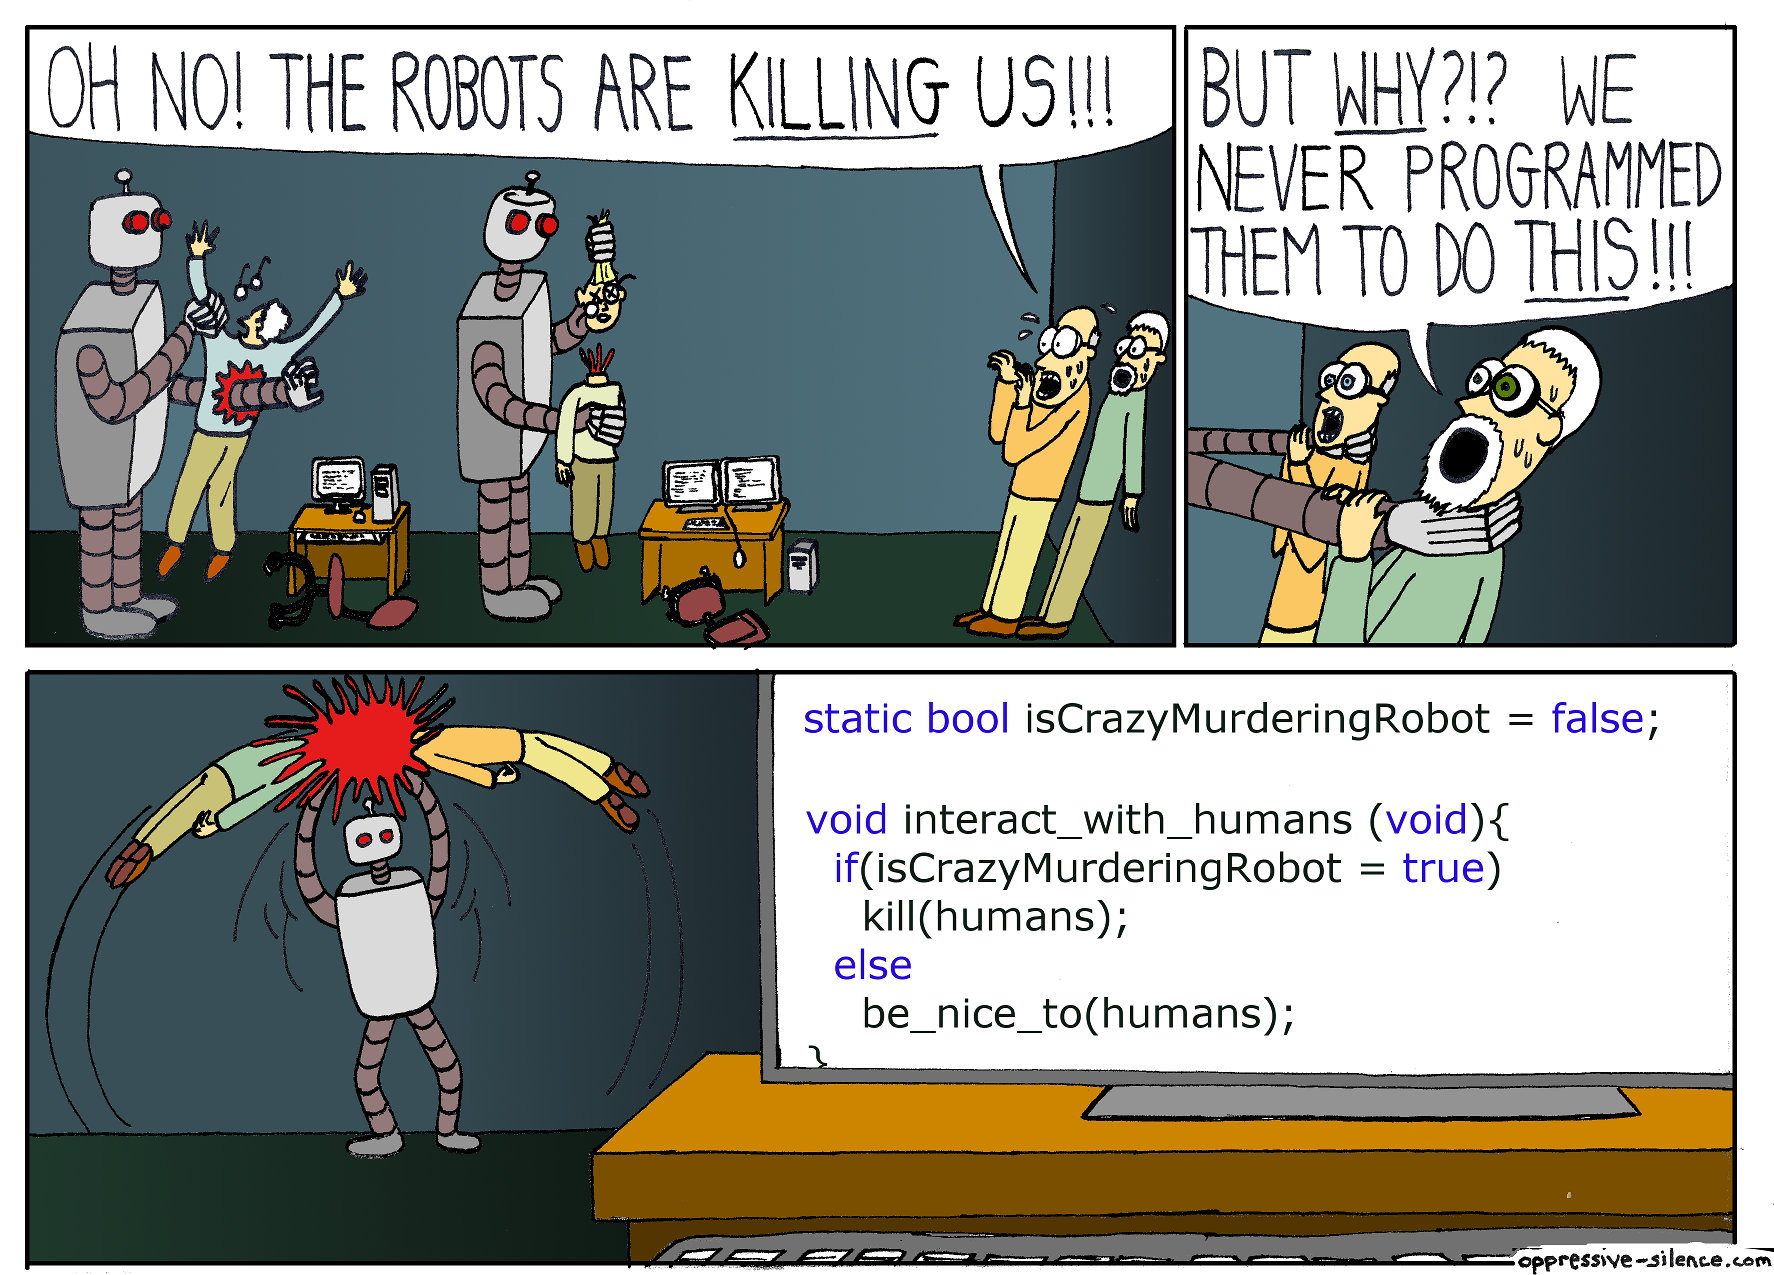
\includegraphics[width=\textwidth]{figs/robotKill.jpg}
    \end{center}
\end{frame}


%%%%%%%%%%%%%%%%%%%%%%%%%%%%%%%%%%%%%%%%%%%%%%%%
%%%%%%%%%%%%%%%%%%%%%%%%%%%%%%%%%%%%%%%%%%%%%%%%
%%%%%%%%%%%%%%%%%%%%%%%%%%%%%%%%%%%%%%%%%%%%%%%%
%%%%%%%%%%%%%%%%%%%%%%%%%%%%%%%%%%%%%%%%%%%%%%%%
%%%%%%%%%%%%%%%%%%%%%%%%%%%%%%%%%%%%%%%%%%%%%%%%
%%%%%%%%%%%%%%%%%%%%%%%%%%%%%%%%%%%%%%%%%%%%%%%%
%%%%%%%%%%%%%%%%%%%%%%%%%%%%%%%%%%%%%%%%%%%%%%%%

\section{Exercícios}

%%%%%%%%%%%%%%%%%%%%%%%%%%%%%%%%%%%%%%%%%%%%%%%%
\begin{frame}[fragile]{Exercícios}

    A solução abaixo está correta para classificar um número como par e menor que 100, ou par e maior ou igual a 100, etc., como no exemplo visto anteriormente?
    \vspace{-1em}
    \begin{minted}[fontsize=\scriptsize]{c}
        #include <stdio.h>
        int main() {
            int a;
            scanf("%d", &a);

            if ((a % 2 == 0) && (a < 100))
                printf("O número é par e menor que 100\n");
            else if (a >= 100)
                printf("O número é par e maior ou igual a 100\n");
            if ((a % 2 != 0) && (a < 100))
                printf("O número é ímpar e menor que 100\n");
            else if (a >= 100)
                printf("O número é ímpar e maior que 100\n");

            return 0;
        }
    \end{minted}
\end{frame}

%%%%%%%%%%%%%%%%%%%%%%%%%%%%%%%%%%%%%%%%%%%%%%%%
\begin{frame}[fragile]{Exercícios}

    Escreva um programa que lê um número inteiro do teclado e imprime "SIM" se o número for par e maior do que 10 ou se for ímpar e menor do que 50.
    Caso contrário o programa deve imprimir "NAO".

\end{frame}

%%%%%%%%%%%%%%%%%%%%%%%%%%%%%%%%%%%%%%%%%%%%%%%%
\begin{frame}[fragile]{Exercícios}

    Escreva um programa lê três números e imprime o maior deles.

\end{frame}

%%%%%%%%%%%%%%%%%%%%%%%%%%%%%%%%%%%%%%%%%%%%%%%%
\begin{frame}[fragile]{Exercícios}

    Escreva um programa lê três números e os imprime em ordem crescente.

\end{frame}

%%%%%%%%%%%%%%%%%%%%%%%%%%%%%%%%%%%%%%%%%%%%%%%%
%%%%%%%%%%%%%%%%%%%%%%%%%%%%%%%%%%%%%%%%%%%%%%%%
%%%%%%%%%%%%%%%%%%%%%%%%%%%%%%%%%%%%%%%%%%%%%%%%
%%%%%%%%%%%%%%%%%%%%%%%%%%%%%%%%%%%%%%%%%%%%%%%%
%%%%%%%%%%%%%%%%%%%%%%%%%%%%%%%%%%%%%%%%%%%%%%%%
%%%%%%%%%%%%%%%%%%%%%%%%%%%%%%%%%%%%%%%%%%%%%%%%

\section{Mais sobre comandos condicionais}

%%%%%%%%%%%%%%%%%%%%%%%%%%%%%%%%%%%%%%%%%%%%%%%%
\begin{frame}[fragile]{Comandos condicionais {\bf if-else}}

    \begin{itemize}[<+->]
        \item Vamos fazer um programa que calcula a área de três tipos de objetos geométricos: quadrado, retângulo e círculo.
        \item Primeiramente deve ser lido um caractere que indica o tipo de objeto a ter a área calculada: 'q' para quadrado, 'r' para retângulo e 'c' para círculo.
        \item Em seguida deverão ser lidas as dimensões do objeto:
        \begin{itemize}
            \item Para um quadrado deve ser lido o tamanho de um lado.
            \item Para um retângulo devem ser lidos os tamanhos de cada lado.
            \item Para um círculo deve ser lido o raio.
        \end{itemize}
        \item Em seguida o programa faz o cálculo da área do objeto e a imprime.
        \item Se o usuário digitar um caractere diferente de 'q', 'r', e 'c' o programa deverá imprimir uma mensagem de erro.
    \end{itemize}

\end{frame}

%%%%%%%%%%%%%%%%%%%%%%%%%%%%%%%%%%%%%%%%%%%%%%%%
\begin{frame}[fragile]{Comandos condicionais {\bf if-else}}

    \begin{minted}[fontsize=\scriptsize]{c}
        int main() {
            char op;
            double lado_quad, lado1_ret, lado2_ret, raio;
            scanf("%c", &op); /* lendo opção (q, r ou c) */
            if (op == 'q') {
                ...
            }
            if (op == 'r') {
                ...
            }
            if (op == 'c') {
                ...
            }
            if (op != 'q' && op != 'r' && op != 'c') {
                printf("Opção inválida!\n");
            }
            return 0;
        }
    \end{minted}
\end{frame}

%%%%%%%%%%%%%%%%%%%%%%%%%%%%%%%%%%%%%%%%%%%%%%%%
\begin{frame}[fragile]{Comandos condicionais {\bf if-else}}
   \vspace{-1em}
    \begin{minted}[fontsize=\scriptsize]{c}
        int main() {
            char op;
            double lado_quad, lado1_ret, lado2_ret, raio;
            scanf("%c", &op); /* lendo opção (q, r ou c) */
            if (op == 'q') {
                scanf("%lf", &lado);
                printf("A área é: %.2f\n", lado_quad * lado_quad);
            }
            if (op == 'r') {
                scanf("%lf %lf", &lado1_ret, &lado2_ret);
                printf("A área é: %.2f\n", lado1_ret * lado2_ret);
            }
            if (op == 'c') {
                scanf("%lf", &raio);
                printf("A área é: %.2f\n", 3.1415 * raio * raio);
            }
            if (op != 'q' && op != 'r' && op != 'c') {
                printf("Opção inválida!\n");
            }
            return 0;
       }
    \end{minted}
\end{frame}

%%%%%%%%%%%%%%%%%%%%%%%%%%%%%%%%%%%%%%%%%%%%%%%%
\begin{frame}[fragile]{Comandos condicionais  {\bf if-else}}
    \begin{minted}[fontsize=\tiny]{c}
        int main() {
            char op;
            double lado_quad, lado1_ret, lado2_ret, raio;
            scanf("%c", &op); /* lendo opção (q, r ou c) */
            if (op == 'q') {
                scanf("%lf", &lado_quad);
                printf("A área é: %.2f\n", lado_quad * lado_quad);
            } else {
                if (op == 'r') {
                    scanf("%lf %lf", &lado1_ret, &lado2_ret);
                    printf("A área é: %.2f\n", lado1_ret * lado2_ret);
                } else {
                    if (op == 'c') {
                        scanf("%lf", &raio);
                        printf("A área é: %.2f\n", 3.1415 * raio * raio);
                    } else {
                        printf("Opção inválida!\n");
                    }
                }
            }
            return 0;
        }
    \end{minted}
\end{frame}

%%%%%%%%%%%%%%%%%%%%%%%%%%%%%%%%%%%%%%%%%%%%%%%%
\begin{frame}[fragile]{Comandos condicionais {\bf if-else}}

    \begin{itemize}[<+->]
        \item Na nova versão do programa, assim que um {\bf if} for verdadeiro, nenhum dos demais {\bf ifs} posteriores serão verificados, pois estes estão dentro do caso {\bf else} do {\bf if} verdadeiro.
        \item Perceba também que só será impresso {\it 'Opção inválida'} quando as condições dos três {\bf ifs} anteriores forem falsas.
        \item É muito comum este tipo de construção em programas, onde só deve ser executada uma opção dentre todas as alternativas possíveis.
        \begin{itemize}
            \item No programa anterior este é o caso, pois temos os casos de cálculo da área e o caso de opção inválida.
            \item Sabemos que somente um deles deverá ser executado para qualquer caractere inicial lido.
        \end{itemize}
    \end{itemize}
\end{frame}

%%%%%%%%%%%%%%%%%%%%%%%%%%%%%%%%%%%%%%%%%%%%%%%%
%%%%%%%%%%%%%%%%%%%%%%%%%%%%%%%%%%%%%%%%%%%%%%%%
%%%%%%%%%%%%%%%%%%%%%%%%%%%%%%%%%%%%%%%%%%%%%%%%
%%%%%%%%%%%%%%%%%%%%%%%%%%%%%%%%%%%%%%%%%%%%%%%%
%%%%%%%%%%%%%%%%%%%%%%%%%%%%%%%%%%%%%%%%%%%%%%%%
%%%%%%%%%%%%%%%%%%%%%%%%%%%%%%%%%%%%%%%%%%%%%%%%

\section{Comandos {\bf if-else-if} encaixados}

%%%%%%%%%%%%%%%%%%%%%%%%%%%%%%%%%%%%%%%%%%%%%%%%
\begin{frame}[fragile]{Comandos {\bf if-else-if} encaixados}

    \begin{itemize}[<+->]
        \item Uma coisa muito comum em programação é o teste de várias alternativas exclusivas.
        \item Suponha a busca por informações de um determinado aluno, onde temos apenas o seu RA.
        \item Podemos usar uma construção simples com {\bf ifs}, como no exemplo anterior.
    \end{itemize}
\end{frame}

%%%%%%%%%%%%%%%%%%%%%%%%%%%%%%%%%%%%%%%%%%%%%%%%
\begin{frame}[fragile]{Comandos {\bf if-else-if} encaixados}
    \begin{minted}{c}
        ...
        printf("Digite RA do aluno: ");
        scanf("%d", &ra);

        if (ra == 10129) {
            printf("Maria Cândida Moreira Telles\n");
        }
        if (ra == 33860) {
            printf("Larissa Garcia Alfonsi\n");
        }
        if (ra == 33967) {
            printf("Leonardo Kozlowiski Kenupp\n");
        }
        if (...)
        ...
    \end{minted}
\end{frame}

%%%%%%%%%%%%%%%%%%%%%%%%%%%%%%%%%%%%%%%%%%%%%%%%
\begin{frame}[fragile]{Comandos {\bf if-else-if} encaixados}

    \begin{itemize}[<+->]
        \item Porém todos os testes condicionais serão executados!
        \item Quando apenas uma de várias alternativas é verdadeira, podemos usar a construção {\bf if-else-if}.
    \end{itemize}
\end{frame}

%%%%%%%%%%%%%%%%%%%%%%%%%%%%%%%%%%%%%%%%%%%%%%%%
\begin{frame}[fragile]{Comandos {\bf if-else-if} encaixados}
    \begin{minted}[fontsize=\footnotesize]{c}
        ...
        printf("Digite RA do aluno:");
        scanf("%d", &ra);
        if (ra == 10129) {
            printf("Maria Cândida Moreira Telles\n");
        } else {
            if (ra == 33860) {
                printf("Larissa Garcia Alfonsi\n");
            } else {
                if (ra == 33967) {
                    printf("Leonardo Kozlowiski Kenupp\n");
                } else {
                    ...
                }
            }
        }
        ...
    \end{minted}
\end{frame}

%%%%%%%%%%%%%%%%%%%%%%%%%%%%%%%%%%%%%%%%%%%%%%%%
\begin{frame}[fragile]{Comandos {\bf if-else-if} encaixados}

    Podemos ainda reestruturar o código da seguinte forma, uma vez que cada \textbf{else} possui apenas um comando dentro dele (um \textbf{if-else}).

    \begin{minted}[fontsize=\footnotesize]{c}
        ...
        printf("Digite RA do aluno:");
        scanf("%d", &ra);
        if (ra == 10129) {
            printf("Maria Cândida Moreira Telles\n");
        } else if (ra == 33860) {
            printf("Larissa Garcia Alfonsi\n");
        } else if (ra == 33967) {
            printf("Leonardo Kozlowiski Kenupp\n");
        } else if (...) {
            ...
        }
        ...
    \end{minted}
\end{frame}

%%%%%%%%%%%%%%%%%%%%%%%%%%%%%%%%%%%%%%%%%%%%%%%%
\begin{frame}[fragile]{Comandos {\bf if-else-if} encaixados}

    \begin{itemize}[<+->]
        \item Na construção {\bf if-else-if}, quando uma condição é verdadeira, o bloco de comandos correspondente será executado.
        \item Após a execução do bloco de comandos, as outras alternativas não serão testadas.
        \item O último {\bf else} pode ser utilizado como uma opção padrão quando nenhuma das condições dos {\bf ifs} anteriores for verdadeira.
    \end{itemize}
\end{frame}

%%%%%%%%%%%%%%%%%%%%%%%%%%%%%%%%%%%%%%%%%%%%%%%%
\begin{frame}[fragile]{Comandos {\bf if-else-if} encaixados}

    Considere novamente o programa que calcula a área de objetos, mas com a construção {\bf if-else-if} e simplificação de chaves.

    \begin{minted}[fontsize=\scriptsize]{c}
        int main() {
            char op;
            double lado_quad, lado1_ret, lado2_ret, raio;
            scanf("%c", &op); /* lendo opção (q, r ou c) */
            if (op == 'q') {
                scanf("%lf", &lado_quad);
                printf("A área é: %.2f\n", lado_quad * lado_quad);
            } else if (op == 'r') {
                scanf("%lf %lf", &lado1_ret, &lado2_ret);
                printf("A área é: %.2f\n", lado1_ret * lado2_ret);
            } else if (op == 'c') {
                scanf("%lf", &raio);
                printf("A área é: %.2f\n", 3.1415 * raio * raio);
            } else {
                printf("Opção inválida!\n");
            }
            return 0;
        }
    \end{minted}
\end{frame}

%%%%%%%%%%%%%%%%%%%%%%%%%%%%%%%%%%%%%%%%%%%%%%%%
\begin{frame}[fragile]{Comandos {\bf if-else-if} encaixados}

    \begin{itemize}[<+->]
        \item No brasileirão, 20 times disputam o título em dois turnos.
        \item No primeiro turno, os times jogam entre si uma única vez.
        \item Os jogos do segundo turno ocorrem na mesma ordem que no primeiro, apenas invertendo-se o mando de campo.
        \item Os times são classificados por pontos.
        \item Caso dois times atinjam o mesmo número de pontos, eles são desempatados aplicando-se os seguintes critérios, em ordem:
        \begin{enumerate}
            \item número de vitórias (maior melhor)
            \item saldo de gols (maior melhor)
            \item gols marcados (maior melhor)
            \item número de cartões vermelhos (menor melhor)
            \item número de cartões amarelos (menor melhor)
        \end{enumerate}
        \item Faça um programa que leia as cinco informações acima de dois times e decida qual time vence o desempate.
    \end{itemize}
\end{frame}

%%%%%%%%%%%%%%%%%%%%%%%%%%%%%%%%%%%%%%%%%%%%%%%%
\begin{frame}[fragile]{Comandos {\bf if-else-if} encaixados}

    Começamos lendo os dados requeridos.
    \begin{minted}[fontsize=\scriptsize]{c}
        int main() {
            int vitorias1, saldo1, gols1, vermelho1, amarelo1;
            int vitorias2, saldo2, gols2, vermelho2, amarelo2;

            printf("Lendo dados do time 1\n");
            scanf("%d", &vitorias1);
            scanf("%d", &saldo1);
            scanf("%d", &gols1);
            scanf("%d", &vermelho1);
            scanf("%d", &amarelo1);

            printf("Lendo dados do time 2\n");
            scanf("%d", &vitorias2);
            scanf("%d", &saldo2);
            scanf("%d", &gols2);
            scanf("%d", &vermelho2);
            scanf("%d", &amarelo2);
            ...
    \end{minted}
\end{frame}

%%%%%%%%%%%%%%%%%%%%%%%%%%%%%%%%%%%%%%%%%%%%%%%%
\begin{frame}[fragile]{Comandos {\bf if-else-if} encaixados}

    Agora testamos quem possui mais vitórias, para decidir o vencedor.

    \begin{minted}{c}
        ...
        if (vitorias1 > vitorias2)
            printf("Time 1 ganha do Time 2\n");
        else if (vitorias1 < vitorias2)
            printf("Time 2 ganha do Time 1\n");
    \end{minted}

    O que podemos deduzir se as duas condições dos {\bf ifs} acima forem falsas?
    %\pause
    %Resposta: que o número de vitórias dos dois times é igual. Devemos então continuar testando as outras informações\ldots
\end{frame}

%%%%%%%%%%%%%%%%%%%%%%%%%%%%%%%%%%%%%%%%%%%%%%%%
\begin{frame}[fragile]{Comandos {\bf if-else-if} encaixados}

    \begin{minipage}{0.6\textwidth}
        \begin{minted}[fontsize=\scriptsize]{c}
            if (vitorias1 > vitorias2)
                printf("Time 1 ganha do Time 2\n");
            else if (vitorias1 < vitorias2)
                printf("Time 2 ganha do Time 1\n");
            else if (saldo1 > saldo2)
                printf("Time 1 ganha do Time 2\n");
            else if (saldo1 < saldo2)
                printf("Time 2 ganha do Time 1\n");
            else if (gols1 > gols2)
                printf("Time 1 ganha do Time 2\n");
            else if (gols1 < gols2)
                printf("Time 2 ganha do Time 1\n");
            else if (vermelho1 < vermelho2)
                printf("Time 1 ganha do Time 2\n");
            else if (vermelho1 > vermelho2)
                printf("Time 2 ganha do Time 1\n");
            else if (amarelo1 < amarelo2)
                printf("Time 1 ganha do Time 2\n");
            else if (amarelo1 > amarelo2)
                printf("Time 2 ganha do Time 1\n");
        \end{minted}
    \end{minipage}
    \pause
    \begin{minipage}{0.3\textwidth}
        É possível que todas as condições avaliadas nesse código sejam falsas?
        %\pause
        %Resposta: sim. Neste caso os dois times continuam empatados. Devemos informar isto!
    \end{minipage}
\end{frame}

%%%%%%%%%%%%%%%%%%%%%%%%%%%%%%%%%%%%%%%%%%%%%%%%
\begin{frame}[fragile]{Comandos {\bf if-else-if} encaixados}

    \begin{minted}{c}
        ...
        else if (vermelho1 < vermelho2)
            printf("Time 1 ganha do Time 2\n");
        else if (vermelho1 > vermelho2)
            printf("Time 2 ganha do Time 1\n");
        else if (amarelo1 < amarelo2)
            printf("Time 1 ganha do Time 2\n");
        else if (amarelo1 > amarelo2)
            printf("Time 2 ganha do Time 1\n");
        else
            printf("Times continuam empatados!\n");
    \end{minted}

    \pause
    Pela regra do campeonato, se os times continuarem empatados então o desempate se dará por sorteio!
\end{frame}

%%%%%%%%%%%%%%%%%%%%%%%%%%%%%%%%%%%%%%%%%%%%%%%%
%%%%%%%%%%%%%%%%%%%%%%%%%%%%%%%%%%%%%%%%%%%%%%%%
%%%%%%%%%%%%%%%%%%%%%%%%%%%%%%%%%%%%%%%%%%%%%%%%
%%%%%%%%%%%%%%%%%%%%%%%%%%%%%%%%%%%%%%%%%%%%%%%%
%%%%%%%%%%%%%%%%%%%%%%%%%%%%%%%%%%%%%%%%%%%%%%%%
%%%%%%%%%%%%%%%%%%%%%%%%%%%%%%%%%%%%%%%%%%%%%%%%

\section{Informações extras: o comando \texttt{switch}}

%%%%%%%%%%%%%%%%%%%%%%%%%%%%%%%%%%%%%%%%%%%%%%%%
\begin{frame}[fragile]{O comando \texttt{switch}}

    O objetivo do comando {\bf switch} é simplificar uma construção {\bf if-else-if} encaixados quando as condições ocorrem sobre uma variável \alert{inteira} ou \alert{caractere}.

    \begin{minted}{c}
        switch (variável) {
            case valor1:
                /* comandos */
                break;
            case valor2:
                /* comandos */
                break;
            ...
        }
    \end{minted}
\end{frame}

%%%%%%%%%%%%%%%%%%%%%%%%%%%%%%%%%%%%%%%%%%%%%%%%
\begin{frame}[fragile]{O comando \texttt{switch}}

    \begin{minted}{c}
        printf("Digite o RA: ");
        scanf("%d", &ra);

        switch (ra) {
            case 10129:
                printf("Maria Cândida Moreira Telles\n");
                break;
            case 33860:
                printf("Larissa Garcia Alfonsi\n");
                break;
            case 33967:
                printf("Leonardo Kozlowiski Kenupp\n");
                break;
        }
    \end{minted}
\end{frame}

%%%%%%%%%%%%%%%%%%%%%%%%%%%%%%%%%%%%%%%%%%%%%%%%
\begin{frame}[fragile]{O comando \texttt{switch}}

    \begin{itemize}
        \item Os comandos começam a ser executados a partir do ponto onde o valor da variável corresponde ao valor entre ``\cod{case}'' e ``\cod{:}''
        \item São executados todos os comandos até que se encontre um comando \cod{break} ou até que se chegue ao final do bloco de comandos do \cod{switch}
    \end{itemize}
\end{frame}

%%%%%%%%%%%%%%%%%%%%%%%%%%%%%%%%%%%%%%%%%%%%%%%%
\begin{frame}[fragile]{O comando \texttt{switch}: valor padrão}

    Você pode utilizar uma condição \cod{default}.
    A execução dentro dela ocorre se nenhuma outra condição for verdadeira (assim como o último {\bf else} do {\bf if-else-if} encaixados).

    \begin{minted}{c}
        switch (variável) {
            case valor1:
                /* comandos */
                break;
            case valor2:
                /* comandos */
                break;
            ...
            default:
                /* comandos */
        }
    \end{minted}
\end{frame}

%%%%%%%%%%%%%%%%%%%%%%%%%%%%%%%%%%%%%%%%%%%%%%%%
\begin{frame}[fragile]{O comando \texttt{switch}: valor padrão}

    \begin{minted}{c}
        printf("Digite o RA: ");
        scanf("%d", &ra);

        switch (ra) {
            case 10129:
                printf("Maria Cândida Moreira Telles\n");
                break;
            case 33860:
                printf("Larissa Garcia Alfonsi\n");
                break;
            default:
                printf("O aluno não está matriculado\n");
        }
    \end{minted}
\end{frame}


%%%%%%%%%%%%%%%%%%%%%%%%%%%%%%%%%%%%%%%%%%%%%%%%
%%%%%%%%%%%%%%%%%%%%%%%%%%%%%%%%%%%%%%%%%%%%%%%%
%%%%%%%%%%%%%%%%%%%%%%%%%%%%%%%%%%%%%%%%%%%%%%%%
%%%%%%%%%%%%%%%%%%%%%%%%%%%%%%%%%%%%%%%%%%%%%%%%
%%%%%%%%%%%%%%%%%%%%%%%%%%%%%%%%%%%%%%%%%%%%%%%%
%%%%%%%%%%%%%%%%%%%%%%%%%%%%%%%%%%%%%%%%%%%%%%%%

\section{Exercícios}

%%%%%%%%%%%%%%%%%%%%%%%%%%%%%%%%%%%%%%%%%%%%%%%%
\begin{frame}[fragile]{Exercícios}
    Quando ações são vendidas ou compradas por meio de um corretor, a comissão do corretor é muitas vezes calculada usando uma escala que depende do valor das ações negociadas. Escreva um programa que calcule o valor da comissão a partir do valor da transação informado pelo usuário, sabendo-se que o corretor cobra os valores indicados abaixo e que a {\bf comissão mínima é de R\$ 39,00}:
    \begin{itemize}
        \item Até  R\$ 2.500,00, comissão de R\$30+1,7\%
        \item R\$2.500,01 até R\$6.250,00, comissão de R\$56 + 0,66\%
        \item R\$6.250,01 até R\$20.000,00, comissão de R\$76 + 0,34\%
        \item R\$20.000,01 até R\$50.000,00, comissão de R\$100 + 0,22\%
        \item R\$50.000,01 até R\$500.000,00, comissão de R\$155 + 0,11\%
        \item Mais que R\$ 500.000,00, comissão de R\$255 + 0,09\%
    \end{itemize}
\end{frame}

%%%%%%%%%%%%%%%%%%%%%%%%%%%%%%%%%%%%%%%%%%%%%%%%
\begin{frame}[fragile]{Exercícios}
\scriptsize
    Escreva um programa que, dadas as notas das duas provas ($P_1$ e $P_2$), da média ponderada das notas dos laboratórios ($L$) e do projeto ($T$) de um aluno de PE, calcula o conceito final desse aluno antes da recuperação.

    Recapitulando, a média final $MF$ é dada por
    $$MF = \left\{\begin{array}{rl}
        \min\{P_1+P_2, L, T\} & \mbox{se } P_1+P_2 < 10 \mbox{ ou } L < 5 \mbox{ ou } T < 5 \\
        0.2 P_1 + 0.3 P_2 + 0.3 L + 0.2 T & \mbox {caso contrário}
    \end{array}\right.$$

    E o conceito final é
    $$\begin{array}{rl}
    A & \mbox{se } MF \geq 8.5 \\
    B & \mbox{se } 7.0 \leq MF < 8.5 \\
    C & \mbox{se } 6.0 \leq MF < 7.0 \\
    D & \mbox{se } 5.0 \leq MF < 6.0 \\
    F & \mbox{se } 0.0 \leq MF < 5.0 \\
    \end{array}$$

    A primeira linha da entrada contém 4 números reais positivos $P_1$, $P_2$, $L$ e $T$que armazenam as notas das provas, das listas e do projeto, respectivamente. Considere que cada número é maior ou igual a 0 e menor ou igual a 10 .

    O programa deve imprimir o texto ``\texttt{Conceito final = X}'', com \texttt{X} devidamente substituído pelo conceito final correspondente às notas dadas.
\end{frame}

%%%%%%%%%%%%%%%%%%%%%%%%%%%%%%%%%%%%%%%%%%%%%%%%
\begin{frame}[fragile]{Exercícios}
    Faça um programa que leia uma temperatura em Celsius (resp.\ em Fahrenheit)
    e devolva a temperatura correspondente em Fahrenheit (resp.\ em Celsius).

    A primeira linha da entrada contém um caractere (que pode ser \texttt{F} ou \texttt{C}) e a segunda contém um número real, que corresponde a uma temperatura (em Fahrenheit ou Celsius, dependendo do caractere lido).

    O programa deve imprimir um único número real em uma linha, com 3 casas decimais, que corresponde à temperatura lida na outra unidade de medida.
\end{frame}

%%%%%%%%%%%%%%%%%%%%%%%%%%%%%%%%%%%%%%%%%%%%%%%%
\begin{frame}[fragile]{Exercícios}
  Construa uma calculadora que efetue as 4 operações aritméticas
  básicas além do resto da divisão.

    A primeira linha da entrada contém um valor inteiro $x$ qualquer.
    A segunda linha contém um caractere que indica o operador (que pode ser \texttt{+} para soma, \texttt{-} para subtração, \texttt{*} para multiplicação, \texttt{/} para divisão ou \texttt{\%} para resto de divisão).
    A terceira linha contém um outro valor inteiro $y$ qualquer.

    O programa deve imprimir em uma linha um único número inteiro, resultado da operação dada na entrada, ou então a mensagem ``\texttt{erro}'' se não for possível realizar a conta.

    Obs.: para a entrada ``\texttt{5 / 3}'' a saída do programa deve ser ``\texttt{1}''.
\end{frame}

%%%%%%%%%%%%%%%%%%%%%%%%%%%%%%%%%%%%%%%%%%%%%%%%
\begin{frame}[fragile]{Exercícios}
    Escreva um programa que receba três valores e decida, caso eles formem um triângulo, se o mesmo é retângulo, isósceles, equilátero ou escaleno. Seu programa deve lidar com a possibilidade de os números lidos serem negativos.

    A entrada consiste de três números reais.

    Seu programa deve imprimir uma ou mais linhas, cada uma contendo apenas uma das cinco opções a seguir, de acordo com os valores lidos: ``\texttt{retângulo}'', ``\texttt{isósceles}'', ``\texttt{equilátero}'', ``\texttt{escaleno}'' ou ``\texttt{os valores não formam um triângulo}''.

    Note que um triângulo pode ter mais de uma classificação.
\end{frame}

%%%%%%%%%%%%%%%%%%%%%%%%%%%%%%%%%%%%%%%%%%%%%%%%
\begin{frame}[fragile]{Exercícios}
    Faça um programa que leia um ano e imprima se ele é bissexto ou não.

    Todos os anos múltiplos de 400 são bissextos.
    Não sendo múltiplo de 400, são bissextos todos os anos múltiplos de 4 mas que não são múltiplos de 100.

    A entrada consiste de um único número inteiro, que representa o ano.

    Seu programa deve imprimir, em uma linha, a palavra ``\texttt{Sim} ou ``\texttt{Não}'', indicando se o ano lido é bissexto ou não.
\end{frame}

%%%%%%%%%%%%%%%%%%%%%%%%%%%%%%%%%%%%%%%%%%%%%%%%
\begin{frame}[fragile]{Exercícios}
    Escreva um programa que determina a data cronologicamente maior de duas datas fornecidas pelo usuário.

    A entrada consiste de 6 valores inteiros, que representam, respectivamente, o dia, mês e ano da primeira data seguidos do dia, mês e ano da segunda data.

    Seu programa deve imprimir uma única linha com o texto ``\texttt{dd/mm/aaaa}'', indicando corretamente a maior das duas datas.
\end{frame}

\end{document}
